\documentclass[16pt]{beamer}

\mode<presentation> {
  \usetheme{Berlin}
  \usecolortheme{seahorse}
%   \usetheme{default}
  \setbeamercovered{transparent}
}

\usepackage[utf8x]{inputenc}
\usepackage{listings}
\usepackage{color}
\usepackage{times}
\usepackage{hyperref}
\usepackage{graphicx}
\usepackage{amssymb}
\usepackage{amsmath}


% \usepackage[T1]{fontenc}

\title{Tile Server Optimization Tricks}
\subtitle{How Not To Write Code}

\author{Andrii V. Mishkovskyi,\\
  Cogniance Inc.,\\
  \texttt{amishkovskiy@cogniance.com}}
\date{\today}

\subject{Tile Server Architecture}

\begin{document}

\begin{frame}
  \titlepage
\end{frame}

\begin{frame}
  \tableofcontents
\end{frame}

\section{Looking for bottlenecks}

\subsection{From the outside}

\begin{frame}{HTTP benchmarking tools}
  \begin{itemize}
  \item JMeter
  \item tsung
  \item ApacheBench
  \item http\_load
  \item siege
  \end{itemize}
\end{frame}

\begin{frame}{JMeter}
  \begin{itemize}
  \item Default tool used by our QA team
  \item Powerful beyond my comprehension
  \item But it's not that easy to setup correctly
  \end{itemize}
\end{frame}

\begin{frame}{Tsung}
  \begin{itemize}
  \item Even more featurefull than JMeter
  \item Way harder to interact with, no GUI
  \item All tests are described using XML scenarios
  \item Can scale test run over hundreds of servers for distributed testing
  \item Written in Erlang
  \end{itemize}
\end{frame}

\begin{frame}{ApacheBench}
  \begin{itemize}
  \item Not useful for anything but single URL benchmarks
  \item But that's one powerful tool for sure
  \end{itemize}
\end{frame}

\begin{frame}{Siege and http\_load}
  \begin{itemize}
  \item Simple tools for load testing
  \item Give them file with list of URLs and get short statistics of benchmark
  \end{itemize}
\end{frame}

\subsection{From the inside}

\begin{frame}{Available tools}
  \begin{itemize}
  \item hotshot
  \item profile and cProfile
  \item \texttt{twistd --profile}
  \item pgbench
  \end{itemize}
\end{frame}

\begin{frame}{hotshot}
  \begin{itemize}
  \item Logging profiler
  \item Quite good analysis
  \item Doesn't work with Python threading module (which is used occasionally)
  \end{itemize}
\end{frame}

\begin{frame}{profile/cProfile}
  \begin{itemize}
  \item Full-featured deterministic profiling
  \item Lots of available statistics
  \item Context information is not lost
  \item But this only works for Python code (so Mapnik and PostgreSQL are left out)
  \end{itemize}
\end{frame}

\begin{frame}{Using twistd runner}
  \begin{itemize}
  \item Using \texttt{--profile} and \texttt{--profiler}
    switches in \texttt{twistd}
  \item So, just a wrapper for Python profilers
  \end{itemize}
\end{frame}

\begin{frame}{pgbench}
  \begin{itemize}
  \item The ultimate tool for testing PostgreSQL
  \item Has all the features DBA would need when optimizing specific queries
  \item Unfortunately, I couldn't come up with a scenario to simulate the way Mapnik handles communication with PG
  \end{itemize}
\end{frame}

\section{To the meat}

\subsection{Overall}

\begin{frame}{(Self-imposed) Requirements}
  \begin{itemize}
  \item Performance degradation should be predictable
  \item Performance shouldn't degrade when using cache
  \item Standard deviation should be in 25\% of the mean time (that is, response time should preferably be in normal distribution)
  \end{itemize}
\end{frame}

\begin{frame}{The process}
  \begin{itemize}
  \item Preliminary testing (before QA) is done with siege and http\_load
  \item Hudson running locally also has basic performance tests
  \item QA then goes on with standard JMeter procedures
  \end{itemize}
\end{frame}

\subsection{Profiling tiles API}

\begin{frame}{Reality}
  Tiles are not simple to profile correctly
  \begin{itemize}
  \item If using HTTP benchmark, tile might get ``rendered'' in no time due to metatile rendering approach
  \item From the inside, tiles is a loosely coupled system, with lots of non-blocking code
  \item Adding timefunc for every callback sounds like too much work
  \item How do you calculate network latency in reactor model?
  \end{itemize}
\end{frame}

\begin{frame}{Approach}
  \begin{itemize}
  \item Log freaking everything everywhere
  \item Mark every request with its unique identifier
  \item Write analysis tool
  \item Stare in amusement
  \end{itemize}
\end{frame}

\begin{frame}{Results}
  \begin{itemize}
  \item There's no simple pattern
  \item Sometimes 90\% of the time is spent waiting for PostgreSQL to return data
  \item Sometimes 60\% of the time is spent rendering
  \item Adjacent (meta-)tiles with similar data might have drastically different rendering times
  \item There's no definite bottleneck that we could eliminate
  \item And there's a lot of factors which make benchmarking quite unreliable
  \end{itemize}
\end{frame}

\begin{frame}{Tiles optimization summary}
  \begin{itemize}
  \item No bottlenecks \(\Rightarrow\) optimize everything
  \item \ldots or switch to other data store and/or renderer altogether
  \item No real work on optimizing has been done yet due to harsh reality of life and lack of time
  \end{itemize}
\end{frame}

\subsection{Profiling staticmaps API}

\begin{frame}{Reality}
  \begin{itemize}
  \item Performance degraded in exponential way
  \item Performance degraded starting from 2 users
  \item Health checks hardly worked when under high load
  \end{itemize}
\end{frame}

\begin{frame}{Reasons}
  \begin{itemize}
  \item Porting from blocking (threaded) to non-blocking code was done carelessly
  \item Tile gathering code has been a dull iteration, rather than fire-and-collect approach
  \item Too much overhead when collecting tiles
  \end{itemize}
\end{frame}

\begin{frame}{Staticmaps optimization summary}
  \begin{itemize}
  \item All blocking code has been rewritten from scratch
  \item Overhead been eliminated by localizing gathering of tiles
  \item In-code documentation appeared (it appears quite important when rewriting from scratch)
  \end{itemize}
\end{frame}

\begin{frame}[fragile]{This is what we get!}
  \begin{center}
    \resizebox{40mm}{!}{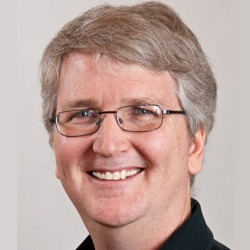
\includegraphics{happy-jim.jpg}}
  \end{center}
\end{frame}

\section*{Summary}

\begin{frame}{Summary}
  \begin{itemize}
  \item It's not always about 20/80 rule
  \item Sometimes there're no apparent bottlenecks
  \item Optimizing one by one is OK, but priorities should be set
  \item Tip: I/O bottlenecks are hard
  \end{itemize}
\end{frame}

\section{Empty section}

\end{document}
